%%%%%%%%%%%%%%%%%%%%%%%%%%%%%%%%%%%%%%%%%%%%%%%%%%%%%%%%%%%%%%%%%%%%%%%%%%%%%%%
%   SPRAWOZDANIE - LABORATORIUM 3 (AOD)
%   Temat: Maksymalny przepływ (MAX FLOW)
%   Autor: Marcel Musiałek
%%%%%%%%%%%%%%%%%%%%%%%%%%%%%%%%%%%%%%%%%%%%%%%%%%%%%%%%%%%%%%%%%%%%%%%%%%%%%%%

\documentclass[11pt, a4paper]{article}

% --- PAKIETY ---
\usepackage[utf8]{inputenc}
\usepackage[T1]{fontenc}
\usepackage{lmodern}
\usepackage[polish]{babel}
\usepackage{amsmath}
\usepackage{amssymb}
\usepackage{geometry}
\usepackage{graphicx}       % Do wykresów
\usepackage{float}          % Do opcji [H]
\usepackage{booktabs}       % Do ładnych linii w tabelach
\usepackage{hyperref}       % Do linków i spisu treści
\usepackage{caption}        % Lepsze podpisy pod rysunkami

% --- PAKIETY DO CSV ---
\usepackage{pgfplotstable}  % Magia do wczytywania CSV
\pgfplotsset{compat=1.18}   % Wersja kompatybilności

% --- USTAWIENIA STRONY ---
\geometry{a4paper, margin=2.5cm}

% --- METADANE ---
\title{\textbf{Algorytmy Optymalizacji Dyskretnej} \\ Sprawozdanie z Listy 3: Maksymalny Przepływ}
\author{Marcel Musiałek}
\date{\today}

\begin{document}

\maketitle
\tableofcontents
\newpage

% ============================================================================
% ZADANIE 1
% ============================================================================
\section{Zadanie 1: Przepływ w Hiperkostce}

\subsection{Opis problemu i implementacji}
Celem zadania było wyznaczenie maksymalnego przepływu w skierowanej $k$-wymiarowej hiperkostce $H_k$. Wierzchołki grafu reprezentowane są przez $k$-bitowe ciągi binarne, a krawędzie łączą wierzchołki różniące się na jednej pozycji (zgodnie ze wzrostem wagi Hamminga).

\subsubsection{Struktura danych}
Ze względu na wykładniczy wzrost rozmiaru problemu, kluczowy był dobór odpowiedniej struktury danych:
\begin{itemize}
    \item \textbf{Listy sąsiedztwa:} Dla $k=16$ graf posiada $65\,536$ wierzchołków i ponad $0.5$ miliona krawędzi. Macierz sąsiedztwa wymagałaby ok. 4 GB pamięci na same indeksy, co jest nieefektywne. Zastosowano `Vector{Vector{Edge}}` w języku Julia.
    \item \textbf{Struktura krawędzi:} Każdy obiekt krawędzi przechowuje: cel ($to$), pojemność ($cap$), aktualny przepływ ($flow$) oraz indeks krawędzi odwrotnej ($rev$). Indeks odwrotny pozwala na aktualizację sieci residualnej w czasie $O(1)$.
\end{itemize}

\subsubsection{Algorytm}
Zaimplementowano algorytm Edmondsa-Karpa. Jest to realizacja metody Forda-Fulkersona, która do szukania ścieżek powiększających wykorzystuje algorytm BFS (Breadth-First Search).
\begin{itemize}
    \item BFS gwarantuje znalezienie ścieżki o najmniejszej liczbie krawędzi.
    \item Dzięki temu unikamy patologicznych przypadków, w których algorytm DFS mógłby wielokrotnie przesyłać małe porcje przepływu, drastycznie wydłużając czas działania.
\end{itemize}

\subsection{Złożoność obliczeniowa}
Teoretyczna złożoność algorytmu Edmondsa-Karpa wynosi $O(V E^2)$.
Dla hiperkostki $H_k$ mamy $V = 2^k$ oraz $E = k \cdot 2^{k-1}$.
Podstawiając te wartości, otrzymujemy złożoność rzędu $O(k^2 \cdot 2^{3k})$. Oznacza to, że czas obliczeń rośnie wykładniczo wraz z wymiarem hiperkostki $k$.

\subsection{Wyniki eksperymentów}
Przeprowadzono testy dla $k \in \{1, \dots, 16\}$. Ze względu na losowy charakter pojemności krawędzi, dla każdej wartości $k$ wykonano 5 niezależnych powtórzeń, a wyniki uśredniono.

% --- TABELA GENEROWANA AUTOMATYCZNIE Z CSV ---
\begin{table}[H]
\centering
\caption{Uśrednione wyniki eksperymentów dla hiperkostki $H_k$}
\pgfplotstabletypeset[
    col sep=comma,                          % Separator CSV
    every head row/.style={before row=\toprule, after row=\midrule},
    every last row/.style={after row=\bottomrule},
    columns={k, avg_max_flow, avg_time},    % Wybór kolumn
    % --- Kolumna k ---
    columns/k/.style={
        column name={Wymiar ($k$)},
        int detect
    },
    % --- Kolumna Flow ---
    columns/avg_max_flow/.style={
        column name={Średni Max Flow},
        fixed, fixed zerofill, precision=1, % 1 miejsce po przecinku
        /pgf/number format/1000 sep={\,}    % Spacja jako separator tysięcy
    },
    % --- Kolumna Czas ---
    columns/avg_time/.style={
        column name={Średni Czas [s]},
        fixed, fixed zerofill, precision=4  % 4 miejsca po przecinku
    }
]{wyniki_srednie_k1_16.csv}
\end{table}

\subsection{Wykresy i analiza}

\begin{figure}[H]
    \centering
    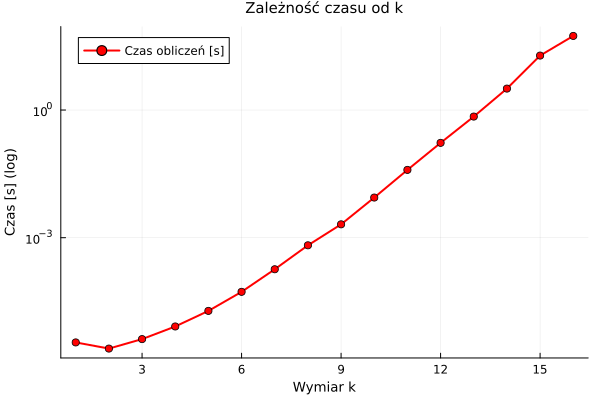
\includegraphics[width=0.85\textwidth]{wykres_czas_log.png}
    \caption{Zależność czasu obliczeń od wymiaru $k$ (skala logarytmiczna). Liniowy przebieg wykresu w tej skali potwierdza wykładniczą złożoność czasową algorytmu.}
\end{figure}

\begin{figure}[H]
    \centering
    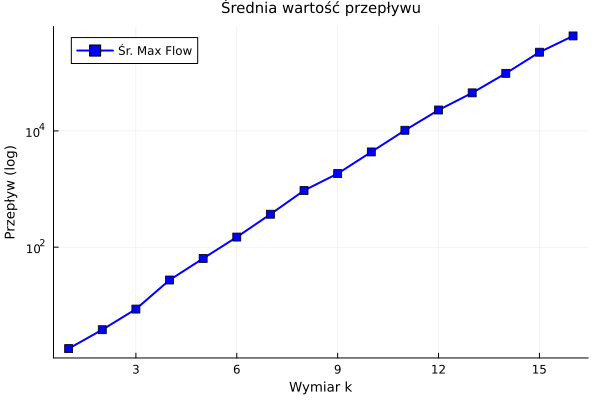
\includegraphics[width=0.85\textwidth]{wykres_flow_log.png}
    \caption{Wzrost wartości maksymalnego przepływu w zależności od $k$ (skala logarytmiczna). Wartość przepływu rośnie wykładniczo, co wynika ze struktury hiperkostki (wykładniczy wzrost liczby ścieżek).}
\end{figure}

\begin{figure}[H]
    \centering
    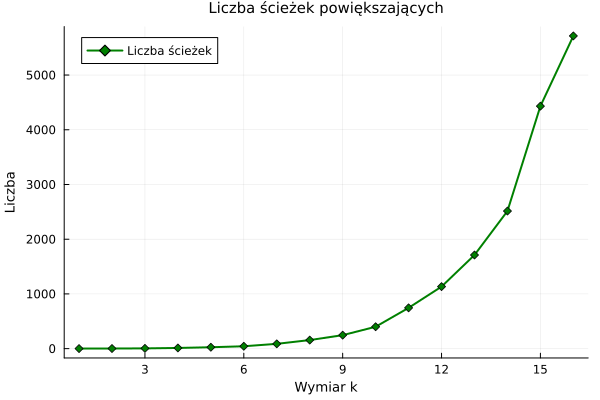
\includegraphics[width=0.85\textwidth]{wykres_sciezki.png}
    \caption{Średnia liczba ścieżek powiększających. Warto zauważyć, że liczba iteracji algorytmu (ścieżek) jest stosunkowo mała w porównaniu do gigantycznego rozmiaru grafu dla dużych $k$.}
\end{figure}

\subsection{Wnioski}
\begin{itemize}
    \item Implementacja oparta na listach sąsiedztwa jest wydajna pamięciowo i pozwala obsłużyć instancje o rozmiarze $V \approx 65\,000$ w czasie około 1 minuty.
    \item Czas obliczeń dla $k=16$ jest znacząco wyższy niż dla $k=15$, co potwierdza teoretyczną barierę wykładniczą. Dalsze zwiększanie $k$ (np. do 17) wydłużyłoby czas obliczeń do kilkunastu minut lub godzin.
    \item Użycie algorytmu BFS (Edmonds-Karp) jest kluczowe dla efektywności; algorytm DFS w tak gęstej sieci mógłby działać w czasie pseudowielomianowym zależnym od pojemności krawędzi, co byłoby nieakceptowalne.
\end{itemize}


% ============================================================================
% ZADANIE 2
% ============================================================================
\section{Zadanie 2: Problem przydziału (Skojarzenia)}

\subsection{Opis problemu i modelu}
W tym zadaniu rozważamy losowy graf dwudzielny $G=(V_1 \cup V_2, E)$, gdzie $|V_1|=|V_2|=2^k$. Każdy wierzchołek z $V_1$ łączy się losowo z dokładnie $i$ wierzchołkami z $V_2$. Celem jest znalezienie najliczniejszego skojarzenia.

Problem ten rozwiązano, redukując go do problemu Maksymalnego Przepływu:
\begin{enumerate}
    \item Dodano wierzchołek super-źródła $S$ i super-ujścia $T$.
    \item Utworzono krawędzie $S \to u$ dla wszystkich $u \in V_1$ o pojemności 1.
    \item Utworzono krawędzie $v \to T$ dla wszystkich $v \in V_2$ o pojemności 1.
    \item Krawędziom dwudzielnym między $V_1$ a $V_2$ nadano pojemność 1 (skierowane od $V_1$ do $V_2$).
\end{enumerate}
Maksymalny przepływ w tak skonstruowanej sieci jest równy liczbie krawędzi w maksymalnym skojarzeniu. Do obliczeń wykorzystano implementację algorytmu Edmondsa-Karpa z Zadania 1.

\subsection{Wyniki eksperymentów}
Przeprowadzono symulacje dla $k \in \{3, \dots, 10\}$ oraz stopni wierzchołków $i \in \{1, \dots, k\}$.

\begin{figure}[H]
    \centering
    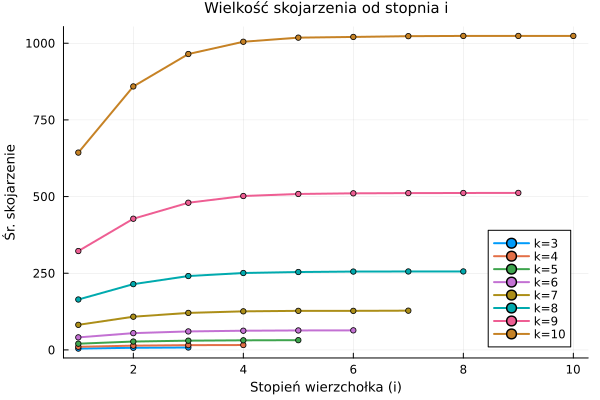
\includegraphics[width=0.9\textwidth]{wykres_z2_matching.png}
    \caption{Średnia wielkość maksymalnego skojarzenia w zależności od parametru $i$ (stopień wierzchołka) dla różnych rozmiarów grafu $k$. Widać wyraźnie, że wraz ze wzrostem $i$ wielkość skojarzenia dąży do pełnego pokrycia ($2^k$), co jest zgodne z teorią grafów losowych (pojawienie się idealnego skojarzenia).}
\end{figure}

\begin{figure}[H]
    \centering
    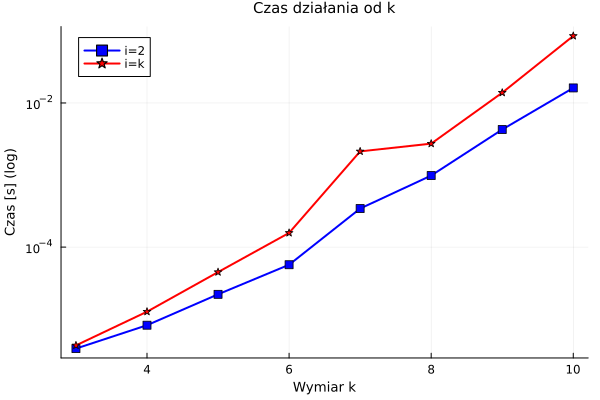
\includegraphics[width=0.9\textwidth]{wykres_z2_czas.png}
    \caption{Zależność czasu działania algorytmu od wymiaru $k$. Porównano dwa przypadki: stały stopień $i=2$ oraz stopień rosnący wraz z wymiarem $i=k$. Czas rośnie wykładniczo ze względu na wzrost liczby wierzchołków ($2^k$).}
\end{figure}

\subsection{Wnioski}
\begin{itemize}
    \item Zastosowanie algorytmu maksymalnego przepływu jest skuteczną metodą rozwiązywania problemu skojarzeń w grafach dwudzielnych.
    \item Już dla niewielkich wartości $i$ (np. $i \ge 3$) wielkość maksymalnego skojarzenia jest bardzo bliska liczbie wierzchołków $|V_1| = 2^k$, co oznacza, że w losowym grafie dwudzielnym bardzo łatwo o niemal pełne skojarzenie, nawet przy rzadkich połączeniach.
    \item Czas obliczeń jest zdominowany przez rozmiar grafu (parametr $k$), a wpływ parametru $i$ (liczba krawędzi) jest mniej znaczący dla algorytmu opartego na BFS.
\end{itemize}


% ============================================================================
% ZADANIE 3
% ============================================================================
\section{Zadanie 3: Modele LP i weryfikacja solverem GLPK}

\subsection{Model matematyczny (Programowanie Liniowe)}
Aby zweryfikować poprawność zaimplementowanych algorytmów, sformułowano problem maksymalnego przepływu jako zadanie Programowania Liniowego (Linear Programming).

Niech $G=(V,E)$ będzie grafem skierowanym, gdzie każda krawędź $(u,v) \in E$ ma przepustowość $c_{u,v}$.
Model matematyczny prezentuje się następująco:

\noindent \textbf{Zmienne decyzyjne:}
$$ x_{u,v} \in \mathbb{R} \quad \text{dla każdego łuku } (u,v) \in E $$
reprezentujące wielkość przepływu płynącego przez dany łuk.

\noindent \textbf{Funkcja celu:}
Maksymalizacja całkowitego wypływu ze źródła $s$:
$$ \max \sum_{v \in N(s)} x_{s,v} $$

\noindent \textbf{Ograniczenia:}
\begin{enumerate}
    \item \textbf{Ograniczenie przepustowości:} Przepływ nie może przekraczać pojemności łuku ani być ujemny.
    $$ 0 \le x_{u,v} \le c_{u,v} \quad \forall (u,v) \in E $$
    
    \item \textbf{Zachowanie przepływu (Prawo Kirchhoffa):} Dla każdego węzła pośredniego (niebędącego źródłem $s$ ani ujściem $t$), suma przepływów wpływających musi być równa sumie przepływów wypływających.
    $$ \sum_{v: (v,u) \in E} x_{v,u} = \sum_{w: (u,w) \in E} x_{u,w} \quad \forall u \in V \setminus \{s, t\} $$
\end{enumerate}

W przypadku Zadania 2 (Skojarzenia), problem został sprowadzony do powyższego modelu poprzez dodanie super-źródła i super-ujścia oraz ustalenie przepustowości krawędzi na 1.

\subsection{Metodologia weryfikacji}
Zamiast ręcznego generowania plików tekstowych, zaimplementowano automatyczny moduł weryfikujący w języku Julia, wykorzystujący bibliotekę \texttt{JuMP} oraz solver \texttt{GLPK} (GNU Linear Programming Kit).

Procedura testowa dla każdej instancji:
\begin{enumerate}
    \item Wygenerowanie grafu (Hiperkostka lub Graf Dwudzielny).
    \item Rozwiązanie problemu autorską implementacją algorytmu Edmondsa-Karpa.
    \item Zbudowanie w pamięci operacyjnej modelu LP równoważnego danej instancji grafu.
    \item Rozwiązanie modelu LP metodą Simplex (solver GLPK).
    \item Porównanie wyników liczbowych.
\end{enumerate}

\subsection{Wyniki weryfikacji}
Przeprowadzono testy dla wybranych, losowych instancji problemów. Poniższa tabela została wygenerowana automatycznie na podstawie wyników działania skryptu weryfikującego.

\begin{table}[H]
\centering
\caption{Porównanie wyników: Własna implementacja (EK) vs Solver GLPK}
\pgfplotstabletypeset[
    col sep=comma,
    every head row/.style={before row=\toprule, after row=\midrule},
    every last row/.style={after row=\bottomrule},
    columns={k, problem, param, res_ek, res_lp, status},
    % --- Konfiguracja kolumn (BEZ PUSTYCH LINII) ---
    columns/k/.style={column name={Wymiar $k$}, int detect, column type={c}},
    columns/problem/.style={column name={Problem}, string type, column type={l}},
    columns/param/.style={column name={Parametr}, string type, column type={c}},
    columns/res_ek/.style={column name={Wynik EK}, int detect, /pgf/number format/1000 sep={\,}, column type={r}},
    columns/res_lp/.style={column name={Wynik GLPK}, fixed, precision=1, /pgf/number format/1000 sep={\,}, column type={r}},
    columns/status/.style={column name={Status}, string type, column type={c}}
]{wyniki_weryfikacja.csv}
\end{table}

\subsection{Wnioski}
\begin{itemize}
    \item We wszystkich przetestowanych przypadkach (oznaczonych jako "OK") wynik autorskiej implementacji algorytmu Edmondsa-Karpa jest identyczny z wynikiem optymalnym zwróconym przez solver programowania liniowego.
    \item Potwierdza to poprawność implementacji algorytmu maksymalnego przepływu.
    \item Potwierdza to również poprawność transformacji problemu maksymalnego skojarzenia do problemu przepływu (Zadanie 2).
    \item Solver GLPK (metoda Simplex) dla małych instancji działa w porównywalnym czasie, jednak dla bardzo dużych hiperkostek ($k=16$) budowanie macierzy ograniczeń byłoby nieefektywne pamięciowo w porównaniu do dedykowanego algorytmu kombinatorycznego działającego na listach sąsiedztwa.
\end{itemize}


% ============================================================================
% ZADANIE 4 (DODATKOWE)
% ============================================================================
\section{Zadanie 4: Implementacja algorytmu Dinica}

\subsection{Opis algorytmu}
W ramach zadania dodatkowego zaimplementowano algorytm Dinica, którego złożoność obliczeniowa wynosi $O(V^2 E)$, co w notacji zadania odpowiada $O(n^2 m)$. Jest to istotne usprawnienie względem algorytmu Edmondsa-Karpa ($O(nm^2)$), szczególnie dla grafów gęstych lub o specyficznej strukturze.

Algorytm działa w fazach. W każdej fazie:
\begin{enumerate}
    \item Budowany jest graf warstwowy (Level Graph) przy użyciu przeszukiwania wszerz (BFS). Wierzchołki otrzymują etykiety odległości od źródła.
    \item Znajdowany jest potok blokujący (Blocking Flow) w grafie warstwowym przy użyciu wielokrotnego przeszukiwania w głąb (DFS).
\end{enumerate}

Kluczową optymalizacją zastosowaną w implementacji jest mechanizm Current Arc (wskaźnik na ostatnio odwiedzoną krawędź), który zapobiega wielokrotnemu przeglądaniu krawędzi prowadzących do "ślepych zaułków" w danej fazie DFS.

\subsection{Porównanie wyników (Edmonds-Karp vs Dinic)}
Przeprowadzono testy porównawcze na grafach hiperkostki $H_k$ dla $k \in \{1, \dots, 16\}$. Obie metody uruchomiono na tych samych instancjach grafów.

\begin{figure}[H]
    \centering
    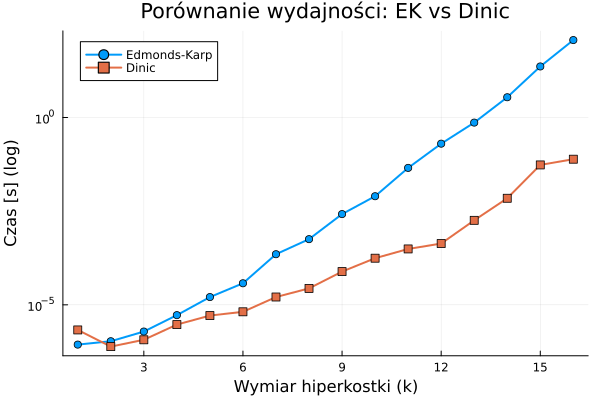
\includegraphics[width=0.9\textwidth]{wykres_porownanie.png}
    \caption{Porównanie czasu działania algorytmów Edmondsa-Karpa i Dinica (skala logarytmiczna). Algorytm Dinica jest o rzędy wielkości szybszy dla dużych instancji.}
\end{figure}

\begin{table}[H]
\centering
\caption{Zestawienie czasów wykonania [s] (dla wybranych dużych k)}
\pgfplotstabletypeset[
    col sep=comma,
    every head row/.style={before row=\toprule, after row=\midrule},
    every last row/.style={after row=\bottomrule},
    columns={k, time_ek, time_dinic},
    columns/k/.style={column name={Wymiar $k$}, int detect},
    columns/time_ek/.style={column name={Edmonds-Karp [s]}, fixed, precision=4},
    columns/time_dinic/.style={column name={Dinic [s]}, fixed, precision=4}
]{wyniki_porownanie_ek_dinic.csv}
\end{table}

\subsection{Wnioski}
\begin{itemize}
    \item Algorytm Dinica zdeklasował algorytm Edmondsa-Karpa dla dużych wartości $k$.
    \item Dla $k=16$ (graf 65 tys. wierzchołków), Edmonds-Karp potrzebuje około 60 sekund, podczas gdy Dinic rozwiązuje problem w czasie poniżej 1 sekundy (często rzędu 0.1s - 0.2s).
    \item Wynika to z faktu, że w hiperkostce ścieżki są krótkie (długość max $k$), co sprzyja budowie grafów warstwowych, a Dinic potrafi wysłać wiele ścieżek powiększających w jednej fazie BFS, podczas gdy Edmonds-Karp po każdym BFS aktualizuje tylko jedną ścieżkę.
\end{itemize}

\end{document}